\documentclass{article}


% load package with some of the available options - you may not need this!
\usepackage[framed,autolinebreaks,useliterate]{mcode}

% for checklist
\usepackage{enumitem,amssymb}
\newlist{todolist}{itemize}{2}
\setlist[todolist]{label=$\square$}
\usepackage{pifont}
\newcommand{\cmark}{\ding{51}}%
\newcommand{\xmark}{\ding{55}}%
\newcommand{\done}{\rlap{$\square$}{\raisebox{2pt}{\large\hspace{1pt}\cmark}}%
\hspace{-2.5pt}}
\newcommand{\wontfix}{\rlap{$\square$}{\large\hspace{1pt}\xmark}}


% something NOT relevant to the usage of the package.
\usepackage{graphicx}
\usepackage{url,textcomp}
\setlength{\parindent}{0pt}
\setlength{\parskip}{18pt}
\title{ECTA Homework 5\\Neuroevolution with the\\Enforced Subpopulations (ESP) algorithm}
\author{\color{red}YOUR NAME, \texttt{your.email@h-brs.de}}
% //////////////////////////////////////////////////

\begin{document}

\maketitle

\begin{center}
	\begin{minipage}{1\linewidth}
		\begin{center}
			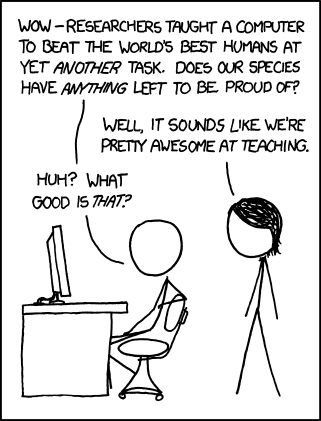
\includegraphics[width=0.7\textwidth]{progeny}
		\end{center}
	\end{minipage}
\end{center}

\newpage

\section{Assignment Description}
	\begin{enumerate}
		\item Solve the following Reinforcement Learning tasks with Neuroevolution.
			\begin{enumerate}
			\item Single Pole Balancing with Velocities
			\item Double Pole Balancing with Velocities
			\item Double Pole Balancing without Velocities
		\end{enumerate}
		\item Compare a standard approach to the ESP algorithm in (c).
	\end{enumerate}

		\begin{itemize}
		\item The task is ``solved'' if the poles does not fall for 1000 time steps.
		\item A 1 and 2 pole balancing simulator function is attached. Given a state and a command it computes the state at the next time step. Examples are included (help: onePole, twoPole). \\\textit{Note:} there is only one 2 pole balancing function, in the case without velocities it is up to you to ``blind'' you ANN of these states, but they are required by the simulator to compute what happens in the next time step.		
		\item You are responsible for all other code, including the ANN.
		\item Additional resources for ESP are available on the LEA
	\end{itemize}

\section{Submission Instructions}
Follow along with the instructions in this PDF, filling in your own code, data, and observations as noted. Your own data should be inserted into the latex code of the PDF and recompiled. All code must be done in MATLAB.

To be perfectly clear we expect two submissions to LEA:
\begin{enumerate}
	\item 1 PDF (report)   -- a modified version of your submission PDF, with your own code snippets, figures, and responses inserted
	\item 1 ZIP (code)     -- a .zip file containing all code use to run experiments (.m files) \textit{and} resulting data as a .mat file
	\item 4 MAT (solution) -- Mat files with the weight matrices of the best found solutions: \textit{spb.mat}, \textit{dpb.mat}, \textit{dpbnv.mat}, and \textit{dpbnv\_esp.mat}
\end{enumerate}





\newpage
\section{The Assignment}

\subsection{Single Pole Balancing (25pts)}
Implement a feed forward network which solves the single pole balancing problem using a fixed topology and a GA or ES (your choice).
\begin{itemize}
	\item (15 pts) Describe your approach. Be sure to mention: the topology of your network, the form of the genotype, the form of the phenotype, the optimization approach used and its details including hyperparameters. Your results should be replicable from your description. Pictures are worth 1000 words.
	\item ( 5 pts) Plot the fitness progress over 10 runs.
	\item ( 5 pts) Upload the weight matrix of your most successful solution in a file called: \textit{spb.mat}
\end{itemize}

\newpage
\subsection{Double Pole Balancing with Velocities (25pts)}
Adapt your feed forward network to solve the double pole balancing problem.
\begin{itemize}
	\item (15 pts) Describe how this approach differs from above. Your results should be replicable from the this description and the one above.
	\item ( 5 pts) Plot the fitness progress over 10 runs.
	\item ( 5 pts) Upload the weight matrix of your most successful solution in a file called: \textit{dpb.mat}
\end{itemize}

\newpage
\subsection{Double Pole Balancing without Velocities (50pts)}
Alter your network topology to solve the double pole balancing problem without velocities using a recurrent neural network. Implement the ESP algorithm to optimize the same network topology. Compare the performance of the two approaches.
\begin{itemize}
	\item (10 pts) Describe how the first approach differs from above. Your results should be replicable from the this description and the one above.
	\item (25 pts) Describe the ESP approach, how it differs from above, and other details, including hyperparameters.
	\item (10 pts) Plot the fitness progress of both approaches over 10 runs, including significance
	\item ( 5 pts) Upload the weight matrix of your most successful solution in 2 files called: \textit{dpbnv.mat} and \textit{dpbnv\_esp.mat}
\end{itemize}

\newpage
\section{Coding an ANN in MATLAB}

\end{document}














